\documentclass{article}
\usepackage[UTF8]{ctex}
\usepackage{amsmath,mathtools,geometry,pgfplots,float,mathrsfs}
\pgfplotsset{compat=1.15}
\usetikzlibrary{arrows}
\geometry{scale=0.7}

\title{每日一题(14.2)}
\author{\kaishu 门宇翎}
\date{2022年4月13日}

\newcommand\parallelogram{\mathord{\text{
\tikz[baseline]\draw (0em, .1ex) -- ++(.9em,0ex) --	++(.2em, 1.2ex) -- ++(-.9em, 0ex) -- cycle;}}}

\begin{document}
\maketitle
\textbf{1. }已知$\parallelogram ABCD$中, $E$为$AB$中点, $AB=10$, $AC=9$, $DE=12$, 求$S_{\parallelogram ABCD}$. {\kaishu(1997年陕西省初中竞赛题)}
\begin{figure}[H]
	\flushright
	\vspace*{-0.5cm}
	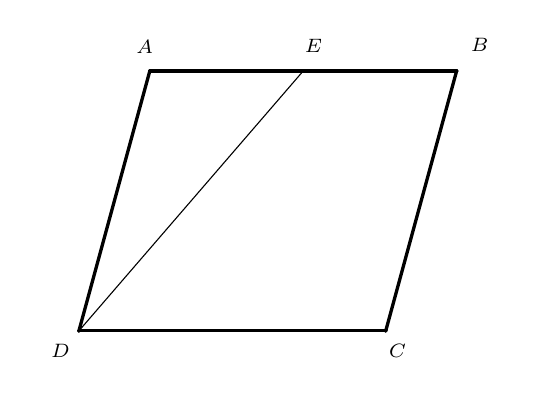
\begin{tikzpicture}[line cap=round,line join=round,>=triangle 45,x=3.0cm,y=3.0cm]
		\clip(-0.21699425034175626,-0.25047847925074174) rectangle (1.8740419685504186,1.2833956010602152);
		\draw [line width=1.2pt] (0.3,1.1)-- (1.598817297684996,1.1);
		\draw [line width=1.2pt] (0.,0.)-- (0.3,1.1);
		\draw [line width=1.2pt] (1.598817297684996,1.1)-- (1.2988172976849959,0.);
		\draw [line width=1.2pt] (1.2988172976849959,0.)-- (0.,0.);
		\draw [line width=0.4pt] (0.,0.)-- (0.949408648842498,1.1);
		\begin{scriptsize}
			\draw [fill=black] (0.3,1.1) circle (0.5pt);
			\draw[color=black] (0.2780745173734858,1.20032474003681) node {$A$};
			\draw [fill=black] (0.,0.) circle (0.5pt);
			\draw[color=black] (-0.07770371569645086,-0.08349765759763428) node {$D$};
			\draw [fill=black] (1.598817297684996,1.1) circle (0.5pt);
			\draw[color=black] (1.6961528520154503,1.2120721345249683) node {$B$};
			\draw [fill=black] (1.2988172976849959,0.) circle (0.5pt);
			\draw[color=black] (1.348765615008484,-0.08349765759763428) node {$C$};
			\draw [fill=black] (0.949408648842498,1.1) circle (0.5pt);
			\draw[color=black] (0.9929873819385473,1.2070375368871862) node {$E$};
		\end{scriptsize}
	\end{tikzpicture}
\end{figure}\vspace*{-0.5cm}\par
\textbf{2. }已知$P$为等腰$\triangle ABC$内一点, $AB=BC$, $\angle BPC=108^\circ$, $D$为$AC$中点, $BP$与$PC$交于$E$. 若$P$为$\triangle ABE$的内心, 求$\angle PAC$. {\kaishu (2014年全国初中数学联赛题)}
\vspace*{-2cm}
\begin{figure}
	\flushright
	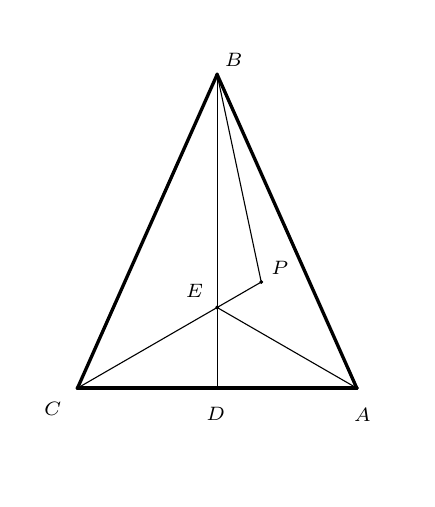
\begin{tikzpicture}[line cap=round,line join=round,>=triangle 45,x=2.5cm,y=2.5cm,]
		\clip(-0.2531537074444294,-0.46271387564511623) rectangle (1.6737342224153502,1.8310064838186453);
		\draw [line width=1.2pt] (0.7093292228999752,1.593179519438245)-- (0.,0.);
		\draw [line width=1.2pt] (0.,0.)-- (1.4186584457999505,0.);
		\draw [line width=1.2pt] (1.4186584457999505,0.)-- (0.7093292228999752,1.593179519438245);
		\draw [line width=0.4pt] (0.7093292228999752,0.4095314177853688)-- (1.4186584457999505,0.);
		\draw [line width=0.4pt] (0.,0.)-- (0.9334209492595018,0.5389108363222094);
		\draw [line width=0.4pt] (0.7093292228999752,1.593179519438245)-- (0.7093292228999754,0.);
		\draw [line width=0.4pt] (0.9334209492595018,0.5389108363222094)-- (0.7093292228999752,1.593179519438245);
		\begin{scriptsize}
			\draw [fill=black] (0.,0.) circle (0.5pt);
			\draw[color=black] (-0.12560658473510086,-0.1051043010022431) node {$C$};
			\draw [fill=black] (0.7093292228999752,1.593179519438245) circle (0.5pt);
			\draw[color=black] (0.7928853754002758,1.6666315565266578) node {$B$};
			\draw [fill=black] (1.4186584457999505,0.) circle (0.5pt);
			\draw[color=black] (1.4478755436935362,-0.13521879149848506) node {$A$};
			\draw [fill=black] (0.7093292228999754,0.) circle (0.5pt);
			\draw[color=black] (0.7025419039115502,-0.13270925062379824) node {$D$};
			\draw [fill=black] (0.9334209492595018,0.5389108363222094) circle (0.5pt);
			\draw[color=black] (1.028782217620837,0.6101148482835032) node {$P$};
			\draw [fill=black] (0.7093292228999752,0.4095314177853688) circle (0.5pt);
			\draw[color=black] (0.594631646300017,0.4921664271732221) node {$E$};
		\end{scriptsize}
	\end{tikzpicture}
\end{figure}
\end{document}